\chapter{Moduli del Software} % Main chapter title

\section*{4.1 \hspace{1cm} Normalizzazione Database}
\subsection*{4.1.1 \hspace{1cm} Schema ER}
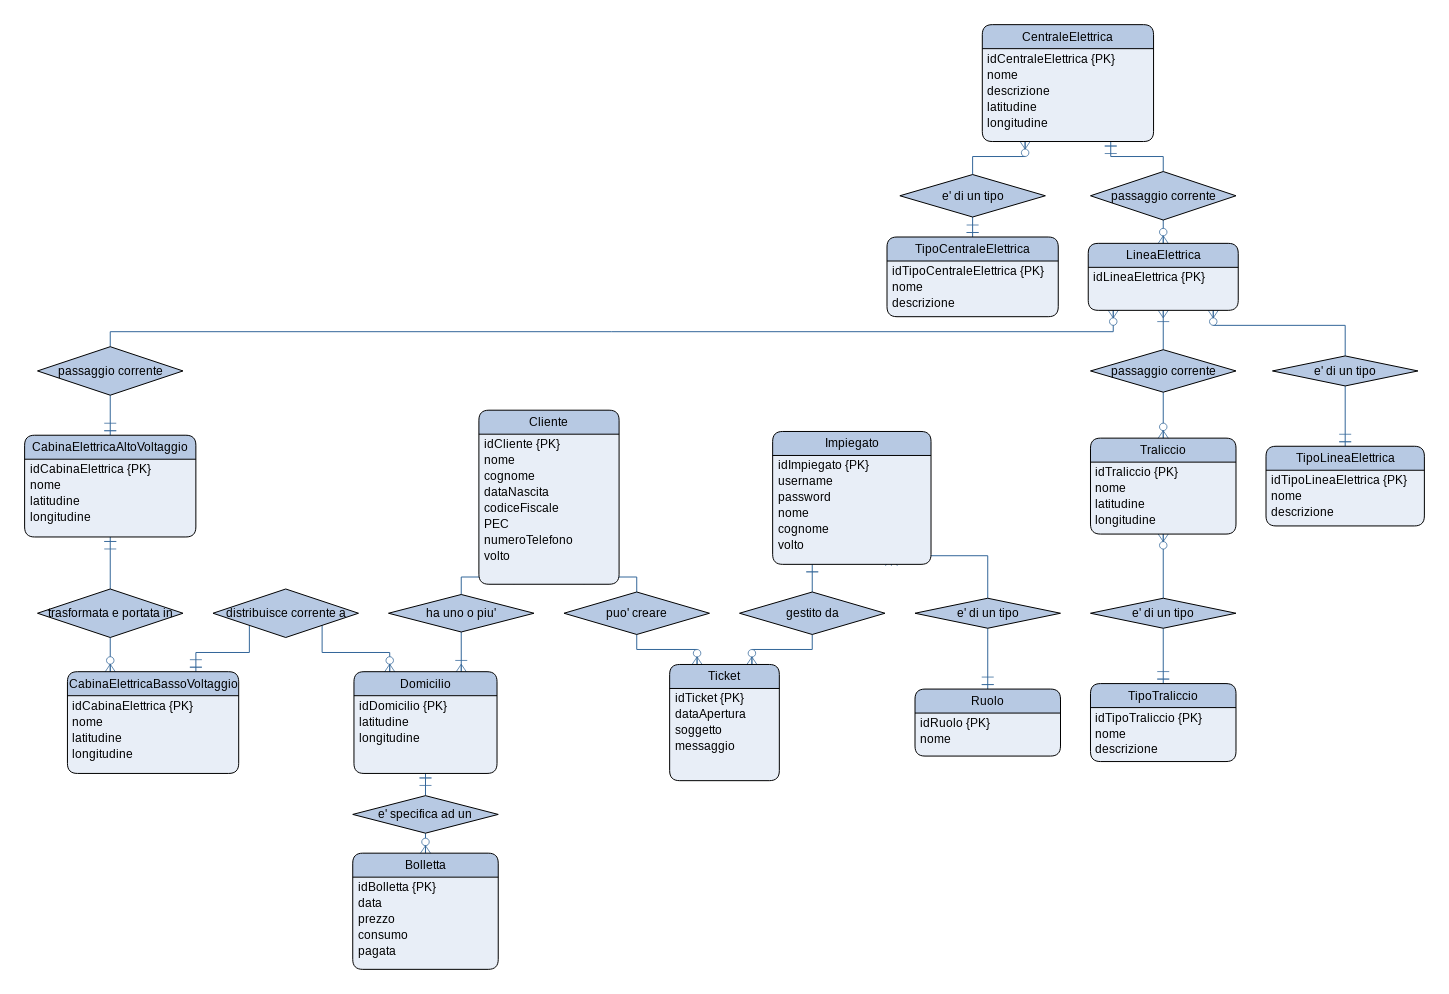
\includegraphics[width=\linewidth]{Figures/ER.png}
\subsection*{4.1.2 \hspace{1cm} 1FN}
Lo schema e' in 1a forma normale in quanto tutti gli attributi sono atomici e dello stesso tipo. \\
La prima forma normale è la più semplice, serve solo rispettare le regole di base per avere questa prima forma, le quali sono:
\begin{itemize}
    \item Utilizzo di campi elementari e non composti
    \item Stesso numero di righe e colonne
    \item Record univoci
\end{itemize}

\subsection*{4.1.3 \hspace{1cm} 2FN}
Dato che non abbiamo chiavi composte, non dobbiamo fare nulla per controllare la 2a forma normale. \\

\subsection*{4.1.3 \hspace{1cm} 3FN}
Tutte le colonne dipendono direttamente dalla chiave primaria, e' ridotto in 3a forma normale. \\

\section*{4.2 \hspace{1cm} Schema Logico}

\begin{center}
    \begin{tabular}{ |l|c|c|c|c|c|c| } 
        \hline
        \multicolumn{7}{|c|}{CentraleElettrica} \\
        \hline
            Name                    & Type      & Size  & Key       & Null  & Default   & Extra \\
        \hline
            idCentrale              & INTEGER   &       & PRIMARY   & NO    &           & AUTO INCREMENT \\
            nome                    & VARCHAR   & 128   &           & NO    &           &                \\
            descrizione             & VARCHAR   & 4096  &           & NO    &           &                \\
            latitudine              & FLOAT     &       &           & NO    &           &                \\
            longitudine             & FLOAT     &       &           & NO    &           &                \\
            idTipoCentraleElettrica & INTEGER   &       & FOREIGN   & NO    &           &                \\
        \hline
    \end{tabular}
\end{center}


\begin{center}
    \begin{tabular}{ |l|c|c|c|c|c|c| } 
        \hline
        \multicolumn{7}{|c|}{LineaElettrica} \\
        \hline
            Name                 & Type     & Size  & Key       & Null  & Default   & Extra \\
        \hline
            idLineaElettrica     & INTEGER  &       & PRIMARY   & NO    &           & AUTO INCREMENT \\
            origine              & INTEGER  &       & FOREIGN   & NO    &           & \\
            destinazione         & INTEGER  &       & FOREIGN   & NO    &           & \\
            idTipoLineaElettrica & INTEGER  &       & FOREIGN   & NO    &           & \\
        \hline
    \end{tabular}
\end{center}

\begin{center}
    \begin{tabular}{ |l|c|c|c|c|c|c| } 
        \hline
        \multicolumn{7}{|c|}{CabinaElettricaAltoVoltaggio} \\
        \hline
            Name             & Type     & Size  & Key       & Null  & Default   & Extra \\
        \hline
            idCabina         & INTEGER  &       & PRIMARY   & NO    &           & AUTO INCREMENT \\
            nome             & VARCHAR  & 128   &           & YES   &           & \\
            latitudine       & FLOAT    &       &           & NO    &           & \\
            longitudine      & FLOAT    &       &           & NO    &           & \\
        \hline
    \end{tabular}
\end{center}

\begin{center}
    \begin{tabular}{ |l|c|c|c|c|c|c| } 
        \hline
        \multicolumn{7}{|c|}{CabinaElettricaBassoVoltaggio} \\
        \hline
            Name                  & Type     & Size  & Key       & Null  & Default   & Extra \\
        \hline
            idCabina              & INTEGER  &       & PRIMARY   & NO    &           & AUTO INCREMENT \\
            nome                  & VARCHAR  & 128   &           & YES   &           & \\
            latitudine            & FLOAT    &       &           & NO    &           & \\
            longitudine           & FLOAT    &       &           & NO    &           & \\
            idCabinaAltoVoltaggio & INTEGER  &       & FOREIGN   & NO    &           & \\
        \hline
    \end{tabular}
\end{center}

\begin{center}
    \begin{tabular}{ |l|c|c|c|c|c|c| } 
        \hline
        \multicolumn{7}{|c|}{PassaggioLinea} \\
        \hline
            Name                    & Type     & Size   & Key       & Null  & Default   & Extra \\
        \hline
            idPassaggio             & INTEGER  &        & PRIMARY   & NO    &           & AUTO INCREMENT \\
            idLinea                 & INTEGER  &        & FOREIGN   & NO    & 1         & \\
            idTraliccioOrigine      & INTEGER  &        & FOREIGN   & SI    &           & \\
            idTraliccioDestinazione & INTEGER  &        & FOREIGN   & SI    &           & \\
        \hline
    \end{tabular}
\end{center}

\begin{center}
    \begin{tabular}{ |l|c|c|c|c|c|c| } 
        \hline
        \multicolumn{7}{|c|}{Traliccio} \\
        \hline
            Name             & Type     & Size  & Key       & Null  & Default   & Extra \\
        \hline
            idTraliccio      & INTEGER  &       & PRIMARY   & NO    &           & AUTO INCREMENT \\
            nome             & VARCHAR  & 64    &           & SI    &           & \\
            latitude         & FLOAT    &       &           & NO    &           & \\
            longitude        & FLOAT    &       &           & NO    &           & \\
            idTipoTraliccio  & INTEGER  &       & FOREIGN   & NO    &           & \\
        \hline
    \end{tabular}
\end{center}

\begin{center}
    \begin{tabular}{ |l|c|c|c|c|c|c| } 
        \hline
        \multicolumn{7}{|c|}{Cliente} \\
        \hline
            Name             & Type     & Size  & Key       & Null  & Default   & Extra \\
        \hline
            idCliente        & INTEGER  &       & PRIMARY   & NO    &           & AUTO INCREMENT \\
            nome             & VARCHAR  & 64    &           & NO    &           & \\
            cognome          & VARCHAR  & 64    &           & NO    &           & \\
            dataNascita      & DATE     &       &           & NO    &           & \\
            codiceFiscale    & VARCHAR  & 16    &           & NO    &           & UNIQUE \\
            numeroTelefono   & VARCHAR  & 16    &           & NO    &           & UNIQUE \\
            PEC              & VARCHAR  & 300   &           & NO    &           & UNIQUE \\
            password         & VARCHAR  & 256   &           & NO    &           & \\
            volto            & BLOB     &       &           & NO    &           & UNIQUE \\
        \hline
    \end{tabular}
\end{center}
\begin{center}
    \begin{tabular}{ |l|c|c|c|c|c|c| } 
        \hline
        \multicolumn{7}{|c|}{Domicilio} \\
        \hline
            Name             & Type     & Size  & Key       & Null  & Default   & Extra \\
        \hline
            idDomicilio                     & INTEGER  &       & PRIMARY   & NO    &           & AUTO INCREMENT \\
            idCliente                       & INTEGER  &       & FOREIGN   & NO    &           & \\
            idCabinaElettricaBassoVoltaggio & INTEGER  &       & FOREIGN   & NO    &           & \\
            latitudine                      & FLOAT    &       &           & NO    &           & \\
            longitudine                     & FLOAT    &       &           & NO    &           & \\
        \hline
    \end{tabular}
\end{center}
\begin{center}
    \begin{tabular}{ |l|c|c|c|c|c|c| } 
        \hline
        \multicolumn{7}{|c|}{Bolletta} \\
        \hline
            Name             & Type     & Size  & Key       & Null  & Default   & Extra \\
        \hline
            idBolletta       & INTEGER  &       & PRIMARY   & NO    &           & AUTO INCREMENT \\
            idDomicilio      & INTEGER  &       & FOREIGN   & NO    &           & \\
            consumoWatt      & FLOAT    &       &           & NO    & 0         & \\
            dataBolletta     & DATE     &       &           & NO    & CURDATE   & \\
            pagata           & BOOLEAN  &       &           & NO    & FALSE     & \\
        \hline
    \end{tabular}
\end{center}
\begin{center}
    \begin{tabular}{ |l|c|c|c|c|c|c| } 
        \hline
        \multicolumn{7}{|c|}{Impiegato} \\
        \hline
            Name             & Type     & Size  & Key       & Null  & Default   & Extra \\
        \hline
            idImpiegato      & INTEGER  &       & PRIMARY   & NO    &           & AUTO INCREMENT \\
            username         & VARCHAR  & 300   &           & NO    &           & UNIQUE \\
            password         & CHAR     & 128   &           & NO    &           & \\
            nome             & VARCHAR  & 64    &           & NO    &           & \\
            cognome          & VARCHAR  & 64    &           & NO    &           & \\
            ruolo            & INTEGER  &       & FOREIGN   & NO    &           & \\
            volto            & BLOB     &       &           & NO    &           & UNIQUE \\
        \hline
    \end{tabular}
\end{center}
\begin{center}
    \begin{tabular}{ |l|c|c|c|c|c|c| } 
        \hline
        \multicolumn{7}{|c|}{Ticket} \\
        \hline
            Name             & Type     & Size  & Key       & Null  & Default   & Extra \\
        \hline
            idTicket         & INTEGER  &       & PRIMARY   & NO    &           & AUTO INCREMENT \\
            dataApertura     & DATETIME &       &           & NO    &           & \\
            soggetto         & VARCHAR  & 300   &           & NO    &           & \\
            messaggio        & VARCHAR  & 8192  &           & NO    &           & \\
            idImpiegato      & INTEGER  &       & FOREIGN   & SI    &           & \\
            idCliente        & INTEGER  &       & FOREIGN   & NO    &           & \\
        \hline
    \end{tabular}
\end{center}

\section*{4.3 \hspace{1cm} DDL}
\subsection*{Metodo Tradizionale}
Questo progetto non usa il metodo "tradizionale" per creare le query SQL. \\
Di seguito, però, mostro le istruzioni DDL per creare il database. \\
\lstinputlisting[language=SQL]{Code/ddl.sql}

\subsection*{Il Metodo di SQLAlchemy}
\begin{verbatim*}
api/code/models.py
\end{verbatim*}

\lstinputlisting[language=Python]{../../../project/api/code/models.py}


Per creare le tabelle del database:
\begin{lstlisting}[language=Python]
# Da qualsiasi parte
db = SQLAlchemy(app)
db.create_db()
\end{lstlisting}


\section*{4.4 \hspace{1cm} Inserimento dei Dati}
\subsection*{Metodo Tradizionale}
\lstinputlisting[language=SQL]{Code/data.sql}

\subsection*{Il Metodo di SQLAlchemy}
\lstinputlisting[language=Python]{../../../project/api/code/data/users.py}


\section*{4.5 \hspace{1cm} Alcune query}
\subsection*{4.5.1 \hspace{1cm} Membri del team "Financing"}
\subsubsection*{Metodo Tradizionale}
\lstinputlisting[language=SQL]{Code/query-1.sql}

\subsubsection*{Il Metodo di SQLAlchemy}
\begin{lstlisting}[language=Python]
User.query.filter_by(role=Role.query.filter_by(name='Finances')[0].id)
\end{lstlisting}


\section*{4.5.2 \hspace{1cm} Centrali Elettriche rinnovabili}
\subsection*{Il Metodo Tradizionale}
\lstinputlisting[language=SQL]{Code/query-2.sql}

\subsubsection*{Il Metodo di SQLAlchemy}
\begin{lstlisting}[language=Python]
    PowerPlant.query.filter(
        PowerPlant.category.in_(
            PowerPlantCategory.query.filter_by(name='Hydro')[0].id,
            PowerPlantCategory.query.filter_by(name='Solar')[0].id,
            PowerPlantCategory.query.filter_by(name='Wind')[0].id,
            PowerPlantCategory.query.filter_by(name='Nuclear')[0].id,
            PowerPlantCategory.query.filter_by(name='Geothermal')[0].id,
        )
    )
\end{lstlisting}
